\chapter{时序图分析模块的设计与实现}
\sys 的时序图分析模块运行在一个单独的分析节点上,同时处理图事务请求和第一类时序图分析任务,它包含的时间数据属于事务时间。
本章将详细介绍一个高效可更新的、基于时序属性图模型的图存储结构\store,然后介绍时序图分析模块使用的基于epoch的粗粒度MVCC机制和\store 结合该机制的修改后版本\newstore,分析这些优化是如何带来读写效率的提升的。
最后将介绍时序图分析模块的只读事务,以及如何基于只读事务在图分析引擎中实现时序图分析算法。

\section{动态图存储结构\store}
图拓扑的CSR表示具有非常好的读性能,但它更新起来非常困难;邻接列表表示的更新效率更高,但它会牺牲读的性能。
为了在实现时序图分析模块的高效图分析性能的同时,保证其良好的图更新效率,本文设计了一个高效的动态图存储\store,它实现了与CSR接近的良好的数据局部性,同时也支持高效的图数据更新。

\begin{figure}[htb]
\center{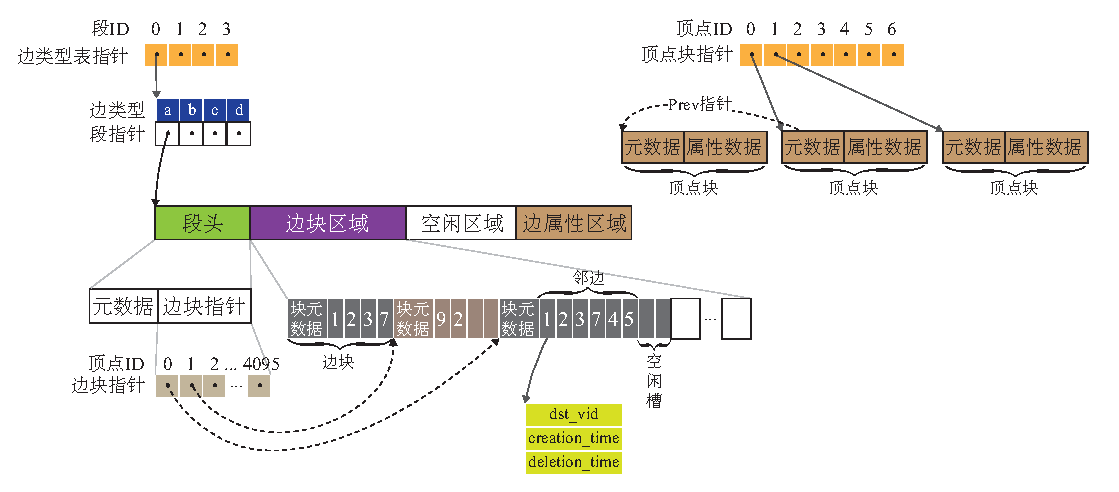
\includegraphics[width=1\textwidth]  {figures/segcsr.eps}} 
\bicaption{动态图存储\store 的结构}{The structure of dynamic graph storage \store}
\label{segcsr}
\end{figure}

\store 的结构如图\ref{segcsr}。\store 使用段来管理固定数量(默认 4096)顶点的所有特定类型的邻边,如果使用\texttt{Seg(sid,type)}表示ID为\texttt{sid}、管理的邻边类型为\texttt{type}的段,那么段\texttt{Seg(0,a)}管理的是ID为 $0-4095$的顶点的所有类型为\texttt{a}的邻边,段\texttt{Seg(1,b)}管理的是ID为$4096-8191$的顶点的所有类型为\texttt{b}的邻边。
\store 使用边类型表\texttt{ETT(sid)}来维护段ID为\texttt{sid}的管理不同邻边类型的段的地址,边类型表的每个表项都是一个边类型到段地址的映射。\store 使用一个边类型表地址数组来维护各边类型表的地址。

一个段由四部分组成,分别是段头、边块区域、空闲区域和边属性区域。段的初始大小是固定的(例如1MB)。段头由两部分组成:段的元数据和指向各顶点边块的指针。段的元数据包括段ID、段大小和已使用段空间大小等。在一个段中,每个顶点都对应一个最新的边块。边块是一块连续的内存区域,由块元数据和边数据区两部分组成。块的元数据包括顶点ID、块大小和已使用块空间大小等。边数据区由描述边信息的结构体组成,该结构体包含三个字段,dst\_vid是边的终点ID,creation\_time是该边的创建时间,deletion\_time是该边的删除时间,它的默认值是INT64\_MAX,表示它还未被删除。边块的初始大小固定,最初被分配出来时会有若干空闲槽,供后续边的插入。如果在插边时发现目标边块的空闲槽已经被用尽,分配器会从空闲区域里分配一个大小为目标边块2倍的新边块,然后把原边块里的数据都迁移到这个新边块里,之后相应顶点的邻边会插入这个新边块中。段头中每个顶点的边块指针指向的是其最新的边块。边块是自段头开始从左往右分配的,而边属性区域是自段尾开始从右往左增长的,边块区域里的边和边属性区域里的边属性数据是对称排布的(如图\ref{edge_property}),块元数据中包含该边块里的边的属性数据在边属性区域中的起始位置。我们要求一个段中各边的属性数据大小相同,以便能够为边块中的空闲槽预留边属性存储空间。

\begin{figure}[htb]
\center{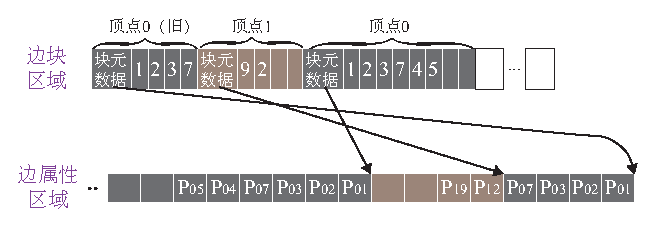
\includegraphics[width=0.7\textwidth]  {figures/edge_property.eps}}
\bicaption{边和边属性数据的对称排布}{Symmetrical layout of edge and edge property data \store}
\label{edge_property}
\end{figure}

如果段的空闲区域不足以分配出新边块和边属性存储空间时,分配器会启动段的迁移过程:分配一个大小为原段二倍的新段,然后按照顶点ID的顺序把原段中每个顶点最新的边块和对应的边属性数据复制到新段里并更新每个顶点的边块指针,最后修改边类型表里的相应地址为新段的地址。

\store 使用顶点块来存储顶点的属性数据,顶点块由元数据区和属性数据区两部分组成,元数据区包含顶点ID、属性数据大小、顶点创建时间和旧顶点块指针等。顶点属性数据更新时,新的顶点块会被创建,其元数据中的旧顶点块指针会指向较旧版本的顶点块,形成一个由不同版本的顶点块组成的链表结构。\store 使用一个顶点块地址数组来维护每个顶点的最新版本顶点块的地址。

\store 使用一个段来管理一定数量的顶点的所有特定类型的邻边,这使得同属于一个段的顶点的边块之间和邻边的属性数据之间都不会离得太远,大大提高了扫边时的数据局部性,从而显著提高扫边性能。段的空闲空间不足时的段迁移操作会按照顶点ID的顺序把原段中每个顶点的边块和邻边的属性数据复制到新段里,使得新段达到近似于CSR的瞬时数据局部性。

绝大多数的并发写问题都可以通过原子操作来解决,例如边块的并发分配可以通过对段头元数据中的已使用段空间大小字段的原子写来实现,对同一边块的并发插入可以通过对块元数据中的已使用块空间大小字段的原子写来实现。
但以下两种并发问题需要使用锁来解决:
\begin{enumerate}
    \item \label{para1} 段迁移过程中的并发问题。考虑以下场景:事务A和事务B在同时往段S中插边,事务A的目标边块有空闲槽,事务B的目标边块没有空闲槽,且段S的空闲区域不足以分配出一个新边块,这时分配器就要为事务B启动段S的迁移,如果段迁移时事务A还未提交(假设系统保证了快照隔离),那么迁移后的段就会丢失事务A插入的边。为了解决这种并发冲突,系统引入了段级别的读写锁:普通的边更新操作只需要尝试获取段的共享锁(读锁),而当该边更新操作会触发段的迁移时,它就会尝试获取段的互斥锁(写锁)。
    \item 边块迁移过程中的并发问题。该问题与\ref{para1}类似,系统使用顶点级别的互斥锁来解决这种并发冲突:边更新操作需要尝试获取起点的互斥锁。
\end{enumerate}

\section{粗粒度的MVCC机制}
MVCC (multi-version concurrency control,多版本并发控制)是一种实现数据库的并发读写的常用方法,它能够避免读操作造成的写操作的阻塞,当数据库中的某个数据值被更新时,MVCC会为该值创建一个新版本,使得并发的读操作可以读到一个稳定的版本。
\store 使用两个时间戳creation\_time和deletion\_time分别表示边的创建时间和删除时间,使用时间戳creation\_time表示顶点的创建时间并使用链表结构将不同版本的顶点块组织起来,以此来实现MVCC。
实时图处理系统通常使用细粒度的MVCC机制,例如LiveGraph使用了组提交策略\cite{grpcmt},每次提交都会将全局写版本号加1,事务的本地写版本号是事务开始时的全局写版本号,它会被用于标识事务所操作数据的版本号。
在图分析场景中,细粒度的MVCC机制是不必要的:图分析是一类相对繁重的计算任务,其执行时间要远远超过一个图事务的执行时间,无需为每次图事务的提交都准备一个不同的版本号,因为图分析任务对细粒度的版本号并不敏感。

为了减少版本数据带来的内存使用和额外计算开销,系统使用了一种基于epoch的粗粒度MVCC机制。
系统会维护一个全局的epoch ID,它从0开始,每隔几十微秒递增一次。
如图\ref{epoch},两个相邻的epoch之间的屏障会使得上一个epoch中的所有事务都完成时,才会开始下一个epoch中事务的执行。
事务的本地写版本号就是其所在epoch的ID,它会被用于标识事务所更新数据的版本号。
同一epoch中的事务可以并行执行,图更新引擎会保证这些事务不会有依赖关系(有依赖关系的事务会按照串行顺序被分配到不同的epoch中执行)。
系统管理员在发起时序图分析任务时需要指定读版本号,时序图分析能够使用的最新稳定版本是\texttt{ceid-1},其中\texttt{ceid}是系统当前的epoch ID。
 
\begin{figure}[htb]
\center{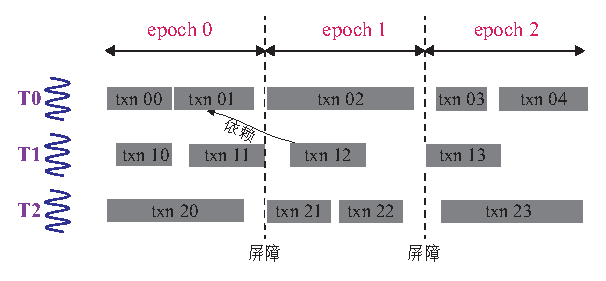
\includegraphics[width=0.6\textwidth]  {figures/epoch.eps}}
\bicaption{epoch屏障示例}{epoch barrier example}
\label{epoch}
\end{figure}

基于上述MVCC机制,我们对\store 的结构进行了调整,使其充分从新的MVCC机制受益,调整后的存储结构称为\newstore。
\newstore 的结构如图\ref{newseg},与\store 相比,它将边块中描述边信息的结构体简化为只包含表示边终点ID的dst\_vid,边块中各边的版本信息(即添加各边的事务的本地写版本号)被统一存储在一个epoch表中。
系统会为段管理的每个顶点都分配一块连续内存作为epoch表,epoch表负责维护顶点的最新边块里的所有边的版本信息,段头会存储每个顶点的epoch表的地址。
边块中的边是只追加的(append-only),相同版本号的边会连续存储,epoch表存储的是每个epoch里添加的第一条边在边块里的逻辑偏移量,例如图\ref{newseg}中顶点0的epoch表的含义就是偏移量为0\textasciitilde 1的边是在epoch 0被插入的,偏移量为2\textasciitilde 4的边是在epoch 3被插入的,偏移量为$5$的边是在epoch 4被插入的。

\begin{figure}[htb]
\center{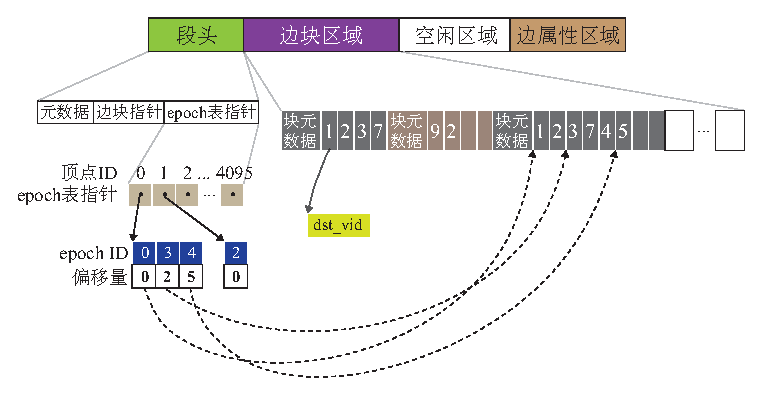
\includegraphics[width=0.9\textwidth]  {figures/newseg.eps}}
\bicaption{\newstore 的结构}{The structure of \newstore}
\label{newseg} 
\end{figure}


\textbf{边的插入。}假设要插入的边是$(u, v)$,其类型为$ty$。
首先通过边类型表地址数组找到边类型表,然后在边类型表中查找类型$ty$对应的表项,即为目标段的地址。
接下来通过目标段的段头中顶点$u$的边块地址即可定位到目标边块,如果目标边块还有空闲槽,则直接把$v$插入第一个空闲槽即可,否则启动边块的迁移,然后再把$v$插入新边块的第一个空闲槽。
边的属性数据要插入边属性区域中的对称位置,相关的元数据(例如块元数据中已使用块空间大小等)也要更新。
如果事务的epoch ID已经存在于顶点$u$对应的epoch表中,则epoch表无需改变,否则需要在epoch表中增加一个表项\texttt{<teid,off>},其中\texttt{teid}就是事务的epoch ID,\texttt{off}是$v$在边块中的偏移量。

\textbf{边的删除。}由于边块中的边数据是只追加的,所以边的删除需要通过边数据的添加来实现。
使用同样的方法定位到目标边块后,通过在边块中添加一个删除标记来记录被删除的边在边块中的偏移量。如果在图分析的扫边过程中遇到删除标记,被删除的边会被直接跳过。

\textbf{垃圾回收。}后台的垃圾回收线程负责过时数据的清理,\newstore 的过时数据包括:
\begin{itemize}
    \item 旧段。段迁移完成后,新段的地址会被注册到边类型表,后续段寻址就会被转移到新段。由于旧段上可能还有未完成的读,所以旧段不能在段迁移完成后就被立即回收。
    垃圾回收线程会监控旧段的使用,旧段上的所有读都完成后,垃圾回收线程就会将其回收。
    \item 被删除的边。为了实现边块的只追加性,系统使用删除标记来记录边的删除。后台的垃圾回收线程会定期对边块中的删除标记进行整理,将删除标记和对应的被删除的边物理地从边块移除。
\end{itemize}

\section{时序图分析算法的实现}
时序图分析模块提供了只读事务RO\_TXN,时序图分析算法都是基于RO\_TXN实现的。表\ref{tab:rotxn}给出了与RO\_TXN相关的接口。

\begin{table}[!hpt]
  \bicaption{RO\_TXN相关接口}{RO\_TXN related interfaces}
  \label{tab:rotxn}
  \centering
  \begin{tabular}{p{7cm}p{5cm}p{2cm}} \toprule
    接口 & 作用 & 类型 \\ \midrule
    \texttt{ROTxn begin\_ROTxn(reid)} & 创建一个读epoch ID为\texttt{reid}的只读事务 & \newstore 的成员函数 \\
    \hline
    \texttt{Seg* locate\_seg(sid,etype)} & 定位段\texttt{Seg(sid,etype)} & \multirow{3}{2cm}{ROTxn的成员函数} \\
    \texttt{EdgeIter get\_edges(segptr,vid)} & 获取地址为\texttt{segptr}的段中顶点\texttt{vid}的邻边的迭代器 \\
    \texttt{sid\_t max\_sid get\_max\_sid()} & 获取最大的段ID \\
    \hline
    \texttt{bool valid()} & 迭代器是否迭代完毕  & \multirow{5}{2cm}{EdgeIter的成员函数} \\
    \texttt{void next()} & 迭代到下一条边 \\
    \texttt{vertex\_t dst\_id()} & 当前边的终点ID \\
    \texttt{string edge\_data()} & 当前边的属性数据 \\
    \texttt{size\_t size()} & 剩余未迭代到的边的数量 \\
    \bottomrule
  \end{tabular}
\end{table}

算法\ref{algo:anademo}使用这些接口实现了一个简单的时序图分析算法,它扫描版本(epoch ID)\texttt{reid}下所有顶点的所有有效邻边,同时把边的属性数据打印出来。首先需要通过begin\_ROTxn接口创建一个读epoch ID为\texttt{reid}的只读事务(第1行),然后使用RO\_Txn提供的get\_max\_sid接口获取该版本下最大的段ID(第2行),接着逐个遍历每个段(3-12行)。在遍历一个段的过程中,需要逐一扫描该段管理的每个顶点的边块:通过RO\_Txn提供的get\_edges接口获取顶点邻边的迭代器(第7行),依次打印迭代到的每条边的属性数据即可(8-12行)。

\begin{algorithm}[htb]
\caption{一个简单的时序图分析算法的实现}
\label{algo:anademo}
\SetKw{KwIn}{in}
\SetKw{KwTo}{to}
\SetKwFunction{Range}{range}
\SetKwFor{For}{for}{\string:}{}
\SetKwIF{If}{ElseIf}{Else}{if}{:}{elif}{else:}{}
\SetKwFor{While}{while}{:}{}
\newcommand{\forcond}{sid = 0 \KwTo{max\_sid}}
\newcommand{\forcondtype}{etype \KwIn{etypes}}
$txn$ = $graph$.begin\_ROTxn($reid$)\;
$max\_sid$ = txn.get\_max\_sid()\;
\For{\forcond}{
    \For{\forcondtype}{
        $segptr$ = txn.locate\_seg($sid$,$etype$)\;
        \For{$vid$ = $sid$ * NUM \KwTo{($sid$ + 1) * NUM - 1}}{
            $iter$ =  $txn$.get\_edges($segptr$,$vid$)\;
            \While{$iter$.valid()}{
                $dst\_id$ = $iter$.dst\_id()\;
                $data$ = $iter$.edge\_data()\;
                print($data$)\;
                $iter$.next()\;
            }
        }
    }
}
\end{algorithm}

目前,时序图分析模块已经实现了多种常用的图分析算法,包括广度优先搜索(BFS)、PageRank、单源最短路径(SSSP)和强连通分量(SCC)等。

\section{本章小结}
本章介绍了\sys 时序图分析模块的设计与实现。系统的时序图分析模块使用了一个高效可更新的、基于时序属性图模型的图存储结构\newstore,它使用段(一块连续的内存空间)来管理固定数量顶点的所有特定类型的邻边,这使得同属于一个段的顶点的边块之间和邻边的属性数据之间都不会离得太远,大大提高了扫边时的数据局部性,从而显著提高扫边性能。为了减少时序数据带来的内存使用和额外计算开销,\newstore 使用了一种基于epoch的粗粒度MVCC机制。最后,时序图分析模块提供了只读事务RO\_TXN,时序图分析算法都是基于 RO\_TXN实现的。